\section{Core Protocol}
\label{sec:coreprotocol}

Consider two fictional users, Alice and Bob. Alice and Bob want to message each other over an untrusted network without leaking any data or metadata to anyone. They use authenticated end-to-end encryption to hide the message content and ensure integrity. They employ two key ideas to hide metadata: sending data at a constant rate and retrieving homomorphically compressed data.

When signing up, each user gets their own \textit{outbox} on the server, which is a dedicated storage space for their messages. Once every minute, Alice sends exactly $1$ KB of data to her outbox. If she has a message to send, she sends the padded encryption of that message. Otherwise, she sends a random sequence of bytes. This simple idea ensures that neither the server nor network observers know when Alice sends a real message.

Our next problem is how to route the message to Bob. In a traditional messaging system, Bob downloads data from Alice's outbox and decrypts it. However, this leaks metadata: the server learns that Bob read from the Alice's outbox.

One solution is for Bob to, once every minute, download \textit{all} outboxes from the server. He can then check the value of Alice's outbox locally. This way, it is impossible for the server to link Alice to Bob.

This simplified scheme is almost how Anysphere works. Unfortunately, Bob cannot download all outboxes every minute — that would be too much data! Instead, he uses \textit{private information retrieval}, a well-studied cryptographic primitive, to compress his download size. \Cref{fig:highlevelpir} illustrates the core protocol. The following subsections will describe the system in detail.

% make this take up both columns at the top of the page
\begin{figure}
    \centering
    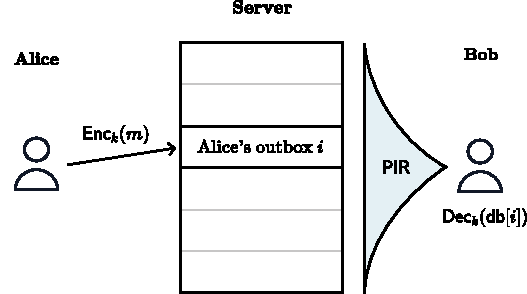
\includegraphics[width=0.7\textwidth]{pirfigure.pdf}
\caption{Alice sends the encryption of a message $m$ to her outbox once every minute. Bob retrieves Alice's outbox using private information retrieval (PIR), which appears to everyone else but Bob as if he had downloaded any outbox. Alice and Bob can use standard symmetric encryption to communicate, and the server will not learn anything at all.}
\label{fig:highlevelpir}
\end{figure}

\subsection{Private information retrieval}

We view the outboxes as an array, called $\db$. Bob wants to download Alice's outbox $\db[i]$ without revealing $i$ to anyone. This problem was first introduced as \textit{private information retrieval} (PIR) in 1995 \cite{chor1995private}, extended in 1997 to our threat model under the name cPIR \cite{kushilevitz1997replication}, and has been extensively studied since then \cite{melchor2016xpir,angel2018pir, ahmad2021addra}.

All known cPIR schemes use homomorphic encryption \cite{gentry2010computing}. To compute the query $q$, Bob encrypts $i$ with a homomorphic encryption scheme using a secret key $s$. That is, $q = \mathsf{HEnc}_s(i)$. The server can then homomorphically evaluate the function $f(i) = \db[i]$, producing the answer $a = \mathsf{HEnc}_s(\db[i])$. Bob can finally decrypt to find $\db[i]$. In practice, $f(i)$ is often defined in terms of a dot product with a unit vector representing $i$, because BFV, the homomorphic scheme being used, \cite{fan2012somewhat}, is particularly good at dot products.

Our implementation currently uses FastPIR, one of the fastest cPIR schemes \cite{ahmad2021addra}. All cPIR schemes have the same security properties, and we are actively researching faster schemes (see \cref{sec:future}).

\subsection{Security}

The simplest version of our core protocol is shown in \cref{fig:simple}. In this section, we show (1) that Alice and Bob enjoy metadata privacy without having to trust anyone else, (2) that our system guarantees message integrity, and (3) that our protocol is resistant to denial of service attacks from users.



% We define security in the simulation sense \cite{lindell2017simulate}. To do so, we first need to define what an attacker learns, which includes both the data sent from all users to the server along with timestamps, as well as the local keys on attacker-controlled devices. Let $(S, i, \mathsf{tk}, c, t)$ represent the data sent to the server in the sending phase at time $t$, let $(R, q, t)$ represent the data sent to the server in the retrieving phase at time $t$, and let $(A, a, t)$ represent the data sent from the server in response to the retrieval request at time $t$. Our protocol does not operate in rounds, so $t$ can be any real number.

% We say that a private communication scheme consists of the four algorithms $(\pcalgostyle{Register}, \mathsf{Send}, \mathsf{Receive}, \mathsf{Route})$, where $\pcalgostyle{Register}$ registers the user and generates a secret key

% \begin{definition}[Metadata privacy]
%     We say that a private communication scheme $(\pcalgostyle{Register}, \mathsf{Send}, \mathsf{Receive}, \mathsf{Route})$ is \textit{metadata-private} if for all $n = n_\lambda = \poly(\lambda)$, all $\mathcal{K} = \mathcal{K}_\lambda \subseteq [n]$, all $T = T_\lambda = \poly(\lambda)$, all user functions $m_u$, $t_u$ and $j_u$, all efficient attackers $\mathcal{S}$, and all efficient distinguishers $\mathcal{A}$, there exists an efficient algorithm $\mathsf{Sim}$, such that the following two probability ensembles, parametrized by $\lambda \in \N$, are computationally indistinguishable:
%     \begin{align*}
%         \Dreal &= \left\{ 
%         \begin{aligned}
%           (\{h_u^T\}_{u \in [n]}, &\{ \sk_u \}_{u \in \calK}, \{ t_u \}_{u \in [n]}) \colon \\
%           \sk_u &\gets \pcalgostyle{Register}(1^\lambda, u) \;\; \forall u \in [n]\\
%           h_u^0 &\gets \emptyset \;\; \forall u \in [n] \\
%           s_u^{i+1} &\gets \mathsf{Send}(m_u(h_u^i), t_u(i), \sk_u) \;\; \forall u \notin \mathcal{K} \\
%           q_u^{i+1} &\gets \mathsf{Retrieve}(j_u(h_u^i), t_u(i), \sk_u) \;\; \forall u \notin \mathcal{K} \\
%           h_u^{i+1} &\gets h_u^i \cup s_u^{i+1} \cup q_u^{i+1}  \cup \mathcal{S}\left(H_t, q_u^{i+1}\right) \;\; \forall u \notin \mathcal{K} \\
%           h_u^{i+1} &\gets h_u^i \cup \mathcal{S}(H_t) \;\; \forall u \in \mathcal{K}
%         \end{aligned}\right\}_{\lambda \in \N}\\
%         \Dideal &= \left\{
%         \begin{aligned}
%           \Sim\big(1^\lambda, \{h_u^T\}_{u \in \calK}, &\{ \sk_u \}_{u \in \calK}, \{ t_u \}_{u \in [n]}\big) \colon \\
%           &(\{h_u^T\}_{u \in [n]}, \{ \sk_u \}_{u \in \calK}, \{ t_u \}_{u \in [n]}) \in \Dreal
%         \end{aligned}
%           \right\}_{\lambda \in \N},
%       \end{align*}
%       where \begin{equation*}
%           H_t = \left\{(\cdot,\ldots,\cdot,t) \in \bigcup_{u, i} h_u^i : t < t_u(i)\right\}
%       \end{equation*}
%       is the global history up until time $t$.
% \end{definition}

% problems with this definition: it is unreadable, Register needs to both register *and* set up all friend connections (which is fine), there is no concept of a message queue which means the m_u needs special requirements, it is both too low-level and too high-level at the same time
% to think about, to get this right: What is the actual API?

\textbf{Going offline.} Users will not always be connected to the internet. At night, most people put their computers to sleep. This means that users will not be sending and receiving exactly once every minute. \xxx{how much information does this leak?} \xxx[stzh]{To ensure security, we urge users to keep a regular transmission schedule by putting their computers asleep at a regular time each day.}

\textbf{Authentication token.} 
On registration, the server creates a unique authentication token for the new user. This allows the server to restrict access to that user's outbox, preventing denial of service attacks from other users. It should still be noted that, in accordance with our threat model, we do not prevent against denial of service attacks by ISPs or the server itself — fundamentally, a powerful actor can always shut down your internet access. In \cref{sec:future} we discuss plans for distributing the server such that, say, only 1 out of 3 servers need to be trusted to provide service.

\begin{figure}
    \begin{framed}
    {\raggedright
        \small
    
    \begin{hangparas}{1em}{1}
    
        \hrule
        \vspace{0.15cm}
        \textsc{\textbf{Protocol $\protocolNumber$: Anysphere Core Protocol}}
        \vspace{0.1cm}
        \hrule
        \vspace{0.1cm}
        \medskip

        \textbf{Registration.}
            Server allocates outbox $i$ and generates authentication token $\authtoken$.
            Alice receives $(i, \authtoken)$.
    
    \medskip

        \textbf{Trust establishment.}
            Alice and Bob agree on a shared secret key $k$. Details in \cref{sec:trustestablishment}.

            \medskip

        \textbf{Sending.}
            Exactly once every minute: \begin{itemize}
                \item If Alice has a queued message $m$: she sends $(i, \authtoken, \enc_k(m))$ to the server, where $k$ is the key shared with Bob.
                \item Otherwise: she sends $(i, \authtoken, r)$ to the server, where $r$ is a random sequence of bytes.
            \end{itemize}
            The server receives $(i, \authtoken, c)$ and stores $c$ in outbox $i$ if $\authtoken$ is correct.

    \medskip

        
        \textbf{Receiving.} Exactly once every minute:
      \begin{itemize}
        \item Bob sends $q = \query(i)$ to the server.
        \item The server responds with $a = \answer(\db, q)$ and Bob decodes it into $c = \decode(a)$.
        \item Bob tries to decrypt $\dec_k(c)$ using the shared secret key $k$.
      \end{itemize}
    \end{hangparas}
    }
    \end{framed}
    \caption{The simplest version of our core protocol.}
    \label{fig:simple}
\end{figure}

\subsection{Multiple contacts}

The simple protocol from before assumed that Alice had a single contact Bob. When Alice has multiple contacts, she picks a message from her queue and encrypts it with the correct key. When Bob has multiple contacts, he randomly picks a contact and retrieves their outbox that round. To make this system more efficient, we prioritize who Bob should retrieve from based on how recently he received messages from his different contacts. 

This way of using the same outbox for all contacts may unfortunately leak some metadata about Alice and Bob's conversation to Alice's other contacts, as described in \cite{angel2018s}. Our threat model assumes that Alice trusts her contacts, which means that this does not compromise security for us. Nevertheless, for users that do not wish to trust their contacts, we plan to give them the option of having multiple outboxes, which would eliminate metadata leakage.

In the future, we are also planning to implement probabilistic batch codes \cite{angel2018pir}, which will make it possible for Bob to retrieve many outboxes at once.

\subsection{Chunks and ACKs}

If Alice wants to send a message longer than 1 KB, she splits the message into 1KB chunks, delivering the chunks to Bob in separate PIR transmissions. To ensure successful delivery, we took inspiration from TCP/IP. Each message from Alice to Bob is labeled with a integer message identifier $m$. Each chunk of message $m$ is further labeled with a sequence number starting from $1$. When Bob receives chunk $c$ of message $m$, he sends Alice a short acknowledgement message $\text{ACK}(m, c)$ over a separate PIR database. Alice listens to Bob's ACK message using PIR, and sends chunk $c + 1$ of message $m$ only after reading $\text{ACK}(m, c)$ from Bob. \Cref{fig:pirandacks} illustrates this.

\begin{figure}
    \centering
    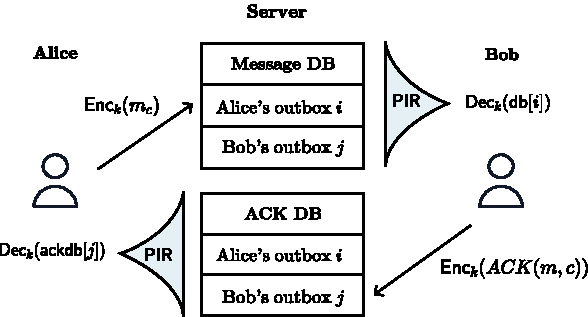
\includegraphics[width=0.7\textwidth]{ACK.pdf}
\caption{All server interactions for a message from Alice to Bob. }
\label{fig:pirandacks}
\end{figure}


Given the limited communication capacity, ACKs turn out to be slightly more subtle than this. In particular, if one user goes offline, we need to continue sending ACKs to them, which could potentially block other ACKs and slow down message transmission. Because each ACK only needs to encode two integers $(m, c)$, we can encode the ACKs for 20 contacts in one database row, which avoids this problem.